\renewcommand{\baselinestretch}{1.2}
\usefonttheme[onlymath]{serif}
\title[Market Power and Contagion]{Market Power and Contagion in Interbank Networks}
\subtitle{An Agent-Based Model of Systemic Risk}

\author{Héctor~Castillo~Andreu}

\institute{
   Departament d'Economia\\
  Universitat Jaume~I
}

\date{19 June 2026}

\subject{Analysis through Agent-Based Models (ABM)}

\pgfdeclareimage[height=.4cm]{university-logo}{img/uji}
\logo{\pgfuseimage{university-logo}}

\AtBeginSection[]
{
  \begin{frame}<beamer>
    \frametitle{Outline}
    \tableofcontents[currentsection]
  \end{frame}
}

\newcommand{\photo}[2][.85]{%
  \begin{center}
    \includegraphics[width=#1\linewidth]{img/#2}
  \end{center}
}

\newcounter{slidenumber}
\newcommand{\frametitlecont}[1]{%
  \frametitle{#1 (\roman{slidenumber})}%
}

%======================================================================
\begin{document}

\setbeamertemplate{footline}{%
  \leavevmode%
  \hbox{%
  \begin{beamercolorbox}[wd=.5\paperwidth,ht=2.5ex,dp=1.125ex,leftskip=.3cm plus1fil,rightskip=.3cm]{author in head/foot}%
    \usebeamerfont{author in head/foot}\insertshortauthor
  \end{beamercolorbox}%
  \begin{beamercolorbox}[wd=.5\paperwidth,ht=2.5ex,dp=1.125ex,leftskip=.3cm,rightskip=.3cm plus1fil]{title in head/foot}%
    \usebeamerfont{title in head/foot}\insertframenumber\,/\,\inserttotalframenumber\ -- \insertshorttitle
  \end{beamercolorbox}}%
  \vskip0pt%
}

\begin{frame}
  \titlepage
\end{frame}

\begin{frame}<handout>[t,allowframebreaks]
  \frametitle{Outline}
  \tableofcontents
\end{frame}

%======================================================================
\section{Abstract}\label{sec:1}
%======================================================================

\begin{frame}{Abstract: ABM, Interbank Market, and Contagion}
  \begin{itemize}
    \item \textbf{Agent-Based Models} to study systemic risk in interbank credit networks.
    \item We examine the relationship between \textbf{network connectivity}, \textbf{market power}, and the propagation of \textbf{bankruptcy cascades}.    
    \item \textbf{Non-monotonic trade-off} between risk sharing and systemic risk---connectivity diversifies risk in normal times but amplifies contagion during crises.
    \item The 2008 financial crisis illustrates how risk-sharing mechanisms can fail under high leverage and heterogeneous agent populations.
  \end{itemize}
\end{frame}

%======================================================================
\section{Risk and Connectivity}\label{sec:2}
%======================================================================

\begin{frame}{The 2008 Crisis: Background}
  \begin{itemize}
    \item Increased bank leverage and corporate debt-equity ratios made the economy fragile.
    \item Standard competitive equilibrium models do not capture the complex interactions that amplify crises.
    \item The interbank market became a \textbf{contagion vector}: failure of one bank triggers a domino effect through interlocking exposures.
  \end{itemize}
\end{frame}

\begin{frame}{The Risk-Sharing Trade-off}
  Two opposing effects of network connectivity:
  \begin{itemize}
    \item \textbf{Benefit:} Increasing connectivity allows \textbf{risk sharing}---banks diversify exposure across more counterparties.
    \item \textbf{Cost:} Excessive connectivity increases \textbf{systemic risk}---default propagates through the network.
    \item Evidence: a \textbf{non-monotonic relationship} exists---low connectivity stabilizes by diluting shocks, but high connectivity facilitates cascading failures.
  \end{itemize}
  %\vspace{0.3cm}
  %``Spreading the risk around the globe may improve stability in good times. However, in times of crisis, critical perturbations can spread across the whole system.'' -- Tedeschi et al.
\end{frame}

% \begin{frame}{Empirical Evidence}
%   \begin{itemize}
%     \item Allen \& Gale (2000), Thurner et al. (2003), Iori et al. (2006): modeling credit systems as random graphs shows that bankruptcy avalanche probability \textbf{decreases} with connectivity.
%     \item Lorenz \& Battiston (2008) show that with \textbf{financial acceleration} (trend reinforcement in fragility), the probability of default does \textbf{not} decrease monotonically with connectivity.
%     \item Iori et al. (2006) identify \textbf{agent heterogeneity} as the root cause of bankruptcy avalanches.
%     %\item Financial crises are characterized by the \textbf{procyclicality of leverage} across institutions.
%     %\item Reserve requirements dampen cascades but \textbf{limit growth} by reducing firm investment.
%   \end{itemize}
% \end{frame}

\begin{frame}{Channels of Contagion in Financial Crises}
  Three primary propagation mechanisms of systemic failure:
  \begin{enumerate}
    \item \textbf{Bank runs:} self-fulfilling panics where depositors withdraw mass funds simultaneously.
    \item \textbf{Asset price contagion:} fire-sale spirals that depreciate assets across the system.
    \item \textbf{Interlocking exposures:} direct linkages through the interbank market---default of one bank triggers defaults in connected banks.
  \end{enumerate}
  \vspace{0.3cm}
  The model distinguishes three failure channels: \textbf{rationing} (borrower cannot secure sufficient funding), \textbf{contagion} (lender suffers losses from borrower default), and \textbf{repayment failure}.
\end{frame}



%======================================================================
\section{Model Framework}\label{sec:3}
%======================================================================

\begin{frame}{Model Overview}
  \begin{itemize}
    \item ABM with $N$ banks in a sequential economy $t = \{0, 1, \dots, T\}$.
    \item Banks connected through an \textbf{Erd\H{o}s--R\'enyi} random graph $G(N, p)$: each edge exists with probability $p$.
    \item Three interacting sectors: goods market, credit market, interbank market.
    \item Goal: analyze how \textbf{connectivity} and \textbf{market power} affect system stability.
  \end{itemize}
\end{frame}

\begin{frame}{Balance Sheet}
  \begin{block}{Accounting Identity}
    $L^t_i + C^t_i + R^t_i = D^t_i + E^t_i$
  \end{block}
  \begin{itemize}
    \item \textbf{Assets:} Long-term loans ($L$), liquidity ($C$), reserves ($R$).
    \item \textbf{Liabilities:} Deposits ($D$), equity ($E$).
    \item Reserves set by regulation: $R_i^t = \hat{r} D_i^t$ with $\hat{r} = 0.02$.
  \end{itemize}
\end{frame}

\begin{frame}{Liquidity Shocks}
  Deposits are exogenously shocked each period:
  \[
    D^t_i = D^{t-1}_i [\mu + \omega \cdot U(0,1)]
  \]
  \begin{itemize}
    \item $\mu$: expected growth rate (0.7).
    \item $\omega$: shock magnitude (0.35).
    \item \textbf{Potential lenders:} banks with positive net deposits (after reserves).
    \item \textbf{Potential borrowers:} banks with negative net deposits exceeding liquidity.
  \end{itemize}
\end{frame}


\begin{frame}{Network Structure}
  \begin{itemize}
    \item Bilateral credit lines formed at the start of each period.
    \item Connectivity controlled by parameter $p$ in the Erd\H{o}s--R\'enyi graph.
    \item Each borrower is matched to \textbf{exactly one} lender per period.
    \item The \textbf{Giant Component Size (GCS)} measures network integration.
  \end{itemize}
\end{frame}

{\usebackgroundtemplate{%
  \vbox to 0pt{\vskip40pt\hbox{\hskip30pt
\includegraphics[width=0.9\paperwidth,height=0.85\paperheight,keepaspectratio]{with_directions.png}}\vss}%
}
\begin{frame}[t]
  \frametitle{Erd\H{o}s--R\'enyi Random Graph}
  \vspace{0.5cm}
  \begin{minipage}{0.85\textwidth}
    \vspace{3.5cm}

    \centering
    \footnotesize
    Each of the $\binom{N}{2}$ possible edges is included independently with probability $p$. For $N=50$ banks:
    \begin{itemize}
      \item $p = 0$: isolated banks, no interbank market.
      \item $p = 1/N = 0.02$: \textbf{percolation threshold}---giant component emerges.
      \item $p > 0.05$: network is saturated ($>92\%$ of banks connected).
    \end{itemize}
  \end{minipage}
\end{frame}
}



\begin{frame}{Network Structure}
The Erd\H{o}s--R\'enyi model does not attempt to replicate the entire interbank market; rather, it illustrates how connection density alters the probability and scale of contagion.
\end{frame}


%======================================================================
\section{Interest Rate and Market Power}\label{sec:4}
%======================================================================


\begin{frame}{Expected Profit}
  Banks are risk-neutral in perfect competition. Expected profit from lending to borrower $j$:
  \begin{block}{}
    $E[\Pi_{i,j}^t] = p_j^t (r_{i,j}^t - m) c_{i,j}^t - (1 - p_j^t) m \cdot c_{i,j}^t$
  \end{block}
  \begin{itemize}
    \item $m$: screening cost ($0.015$).
    \item $p_j^t$: probability of borrower survival.
    \item $r_{i,j}^t$: interest rate; $c_{i,j}^t$: lending capacity.
  \end{itemize}
\end{frame}

\begin{frame}{Interest Rate Derivation}
  Setting $E[\Pi] = 0$ (zero-profit condition):
  \[
    r_{i,j}^t = \frac{m}{p_j^t}
  \]
  Introducing \textbf{market power} $\psi \in [0,1)$:
  \[
    \boxed{r_{i,j}^t = \frac{m}{p_j^t (1 - \psi)}}
  \]
  \begin{itemize}
    \item $\psi = 0$: competitive (actuarially fair) rate.
    \item $\psi > 0$: monopolistic markup from information asymmetry.
  \end{itemize}
\end{frame}

\begin{frame}{Endogenous Market Power}
  Market power evolves endogenously with bank size:
  \[
    \psi_i^t = \frac{E_i^t}{E_i^{t,\max}}
  \]
  \begin{itemize}
    \item Larger banks (higher equity) exercise more market power.
    \item Borrower default probability:
    $p_{b,j}^t = E_j^t / E_j^{t,\max}$.
    \item Leverage: $\lambda_j^t = d_j^t / E_j^t$.
    \item Within the model, market power and default probabilities are determined \textbf{endogenously} from screening costs and shock parameters.
  \end{itemize}
\end{frame}



%======================================================================
\section{Equity and Bankruptcy Dynamics}\label{sec:5}
%======================================================================

\begin{frame}{Equity Evolution}
  \[
    E^t_i = E^{t-1}_i + \sum_{j} l^{t}_{i,j} r^{t}_{i,j} - \sum_{j \subseteq \theta^t_i} \left[ B^{t}_{i,j} - \tilde{L}^t_j \right]
  \]
  \begin{itemize}
    \item \textbf{Bankruptcy:} bank exits if $E_i^t < 0$.
    \item \textbf{Fire sales:} last-resort option (blocked in this model to amplify contagion effects).
    \item Failed banks replaced by new entrants with small initial capital.
  \end{itemize}
\end{frame}


\begin{frame}{Failure Channels}
  Three distinct causes of bank failure:
  \begin{enumerate}
    \item \textbf{Rationing:} borrower cannot secure sufficient funding.
    \item \textbf{Contagion:} lender suffers losses from borrower default (bad debt).
    \item \textbf{Repayment failure:} fully-funded borrower cannot repay loan or interest.
  \end{enumerate}
  \vspace{0.3cm}
  \textbf{Repayment failure dominates} at high connectivity, while rationing dominates at low connectivity.
\end{frame}



%======================================================================
\section{Phase Transition}\label{sec:6}
%======================================================================

\begin{frame}[shrink=0.1]{Phase Transition}
  \begin{itemize}
    \item \textbf{Percolation threshold:} GCS jumps from $\sim 1$ to $\sim 46$ banks ($92\%$).
    \item \textbf{Low $p$:} rationing-dominated, high interest rates, few loans.
    \item \textbf{High $p$:} repayment-failure-dominated, low rates, saturated network.
    \item $p > 0.05$: all macroeconomic metrics stabilize.
  \end{itemize}
\end{frame}

\begin{frame}[shrink=0.1]{Phase Transition}

  \vspace{0.05cm}

  \begin{columns}[T]
    \begin{column}{0.55\textwidth}
      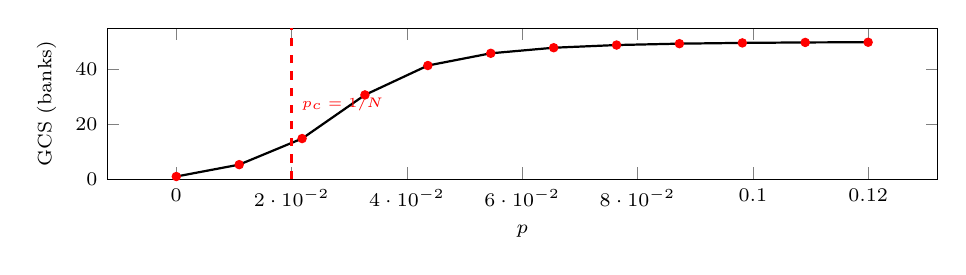
\begin{tikzpicture}
        \begin{axis}[
          width=\textwidth,
          height=3.5cm,
          xlabel={$p$},
          ylabel={GCS (banks)},
          ymin=0, ymax=55,
          font=\scriptsize,
        ]
        \addplot[red, only marks, mark=*, mark size=1.5pt] coordinates {
          (0.00001, 1.01)
          (0.01092, 5.33)
          (0.02183, 14.83)
          (0.03273, 30.72)
          (0.04364, 41.42)
          (0.05455, 45.87)
          (0.06546, 47.90)
          (0.07637, 48.88)
          (0.08727, 49.38)
          (0.09818, 49.66)
          (0.10909, 49.83)
          (0.12000, 49.90)
        };
        \addplot[black, thick] coordinates {
          (0.00001, 1.01)
          (0.01092, 5.33)
          (0.02183, 14.83)
          (0.03273, 30.72)
          (0.04364, 41.42)
          (0.05455, 45.87)
          (0.06546, 47.90)
          (0.07637, 48.88)
          (0.08727, 49.38)
          (0.09818, 49.66)
          (0.10909, 49.83)
          (0.12000, 49.90)
        };
        \draw[red, dashed, thick] (axis cs:0.02,0) -- (axis cs:0.02,55)
          node[pos=0.5, right, font=\tiny]{$p_c = 1/N$};
        \end{axis}
      \end{tikzpicture}
      \vspace{0.1cm}
      \centering
      \textbf{Percolation threshold} for Erd\H{o}s--R\'enyi graph:
      \[
        p_c = \frac{1}{N} = \frac{1}{50} = 0.02
      \]
    \end{column}
    \begin{column}{0.42\textwidth}
      \footnotesize
      \centering
      \begin{tabular}{rr}
        \toprule
        $p$ & GCS \\
        \midrule
        0.00001 & 1 \\
        0.011 & 5 \\
        \textbf{0.022} & \textbf{15} \\
        0.033 & 31 \\
        0.044 & 41 \\
        \textbf{0.055} & \textbf{46} \\
        0.065 & 48 \\
        0.087 & 49 \\
        $\geq 0.11$ & 50 \\
        \bottomrule
      \end{tabular}
    \end{column}
  \end{columns}
\end{frame}


\begin{frame}{Connectivity and Systemic Risk}
  \begin{itemize}
    \item As $p$ increases, the interest rate drops from $30$ (upper bound) to $\sim 1.65$.
    \item Bankruptcies remain stable at $\sim 7$--$7.5$ (limited by model structure).
    \item Active loans saturate at $\sim 13$ ($26\%$ of banks).
    \item Equity jumps from $46.8$ to $\sim 55$ and then plateaus.
    \item Bad debt grows rapidly before stabilizing at $\sim 1.3$.
  \end{itemize}
\end{frame}

%======================================================================
\section{Results}\label{sec:7}
%======================================================================

\begin{frame}{Bankruptcies exposed by the model}
  \begin{columns}[T]
    \begin{column}{0.55\textwidth}
      \centering
      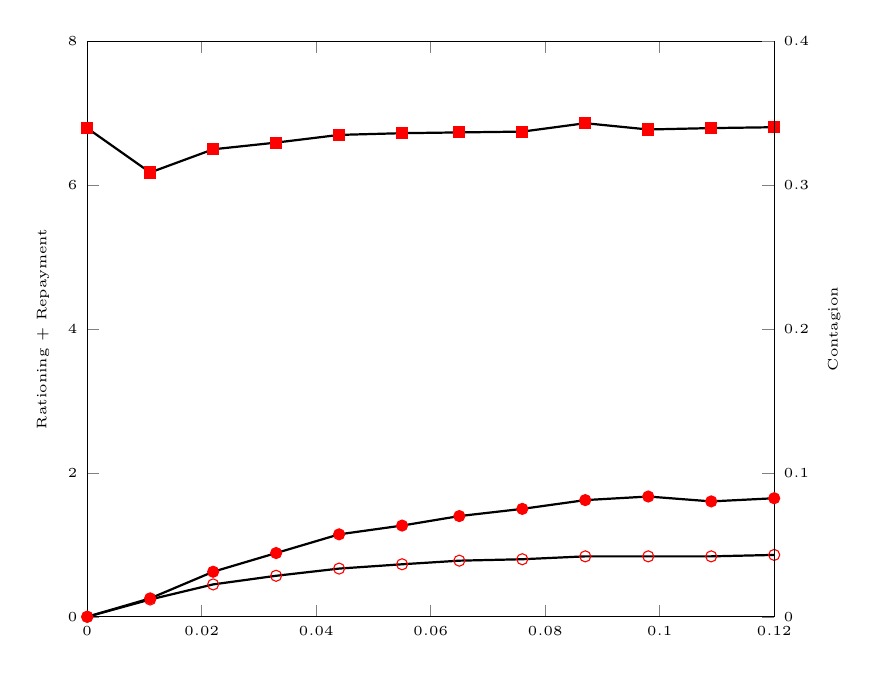
\begin{tikzpicture}
        \begin{axis}[
          width=0.85\textwidth,
          ylabel={Rationing + Repayment},
          ylabel style={font=\tiny},
          ymin=0, ymax=8,
          xmin=0, xmax=0.12,
          xticklabel style={/pgf/number format/fixed, /pgf/number format/precision=2},
          font=\tiny,
        ]
          \addplot[only marks, mark=square*, red] coordinates {
            (0.00001,6.7931)            (0.01100,6.1768)            (0.02200,6.4994)            (0.03300,6.5926)            (0.04400,6.6995)            (0.05500,6.7234)            (0.06500,6.7342)            (0.07600,6.7453)            (0.08700,6.8621)            (0.09800,6.7748)            (0.10900,6.7942)            (0.12000,6.8065)
          };
          \addplot[black, thick]coordinates {
            (0.00001,6.7931)            (0.01100,6.1768)            (0.02200,6.4994)            (0.03300,6.5926)            (0.04400,6.6995)            (0.05500,6.7234)            (0.06500,6.7342)            (0.07600,6.7453)            (0.08700,6.8621)            (0.09800,6.7748)            (0.10900,6.7942)            (0.12000,6.8065)
          };
          \addplot[only marks, mark=o, red] coordinates {
            (0.00001,0.00)            (0.01100,0.24)            (0.02200,0.45)            (0.03300,0.57)            (0.04400,0.67)            (0.05500,0.73)            (0.06500,0.78)            (0.07600,0.80)            (0.08700,0.84)            (0.09800,0.84)            (0.10900,0.84)            (0.12000,0.86)
          };
          \addplot[black, thick]coordinates {
            (0.00001,0.00)            (0.01100,0.24)            (0.02200,0.45)            (0.03300,0.57)            (0.04400,0.67)            (0.05500,0.73)            (0.06500,0.78)            (0.07600,0.80)            (0.08700,0.84)            (0.09800,0.84)            (0.10900,0.84)            (0.12000,0.86)
          };
        \end{axis}
        \begin{axis}[
          width=0.85\textwidth,
          ylabel={Contagion},
          ylabel style={font=\tiny},
          ymin=0, ymax=0.4,
          xmin=0, xmax=0.12,
          axis y line*=right, axis x line=none,
          ylabel near ticks,
          yticklabel style={/pgf/number format/fixed, /pgf/number format/precision=2},
          font=\tiny,
        ]
          \addplot[only marks, mark=*, red] coordinates {
            (0.00001,0.0000)            (0.01100,0.0128)            (0.02200,0.0313)            (0.03300,0.0443)            (0.04400,0.0573)            (0.05500,0.0634)            (0.06500,0.0700)            (0.07600,0.0750)            (0.08700,0.0811)            (0.09800,0.0836)            (0.10900,0.0802)            (0.12000,0.0824)
          };
          \addplot[black, thick]coordinates {
            (0.00001,0.0000)            (0.01100,0.0128)            (0.02200,0.0313)            (0.03300,0.0443)            (0.04400,0.0573)            (0.05500,0.0634)            (0.06500,0.0700)            (0.07600,0.0750)            (0.08700,0.0811)            (0.09800,0.0836)            (0.10900,0.0802)            (0.12000,0.0824)
          };
        \end{axis}
        \end{tikzpicture}
    \end{column}
    \begin{column}{0.43\textwidth}
      \tiny
      \begin{minipage}[t]{0.2\textwidth}
        $\square$ Rat.\par
        $\bullet$ Cont.\par
        $\circ$ Repayment fail.
      \end{minipage}
      \begin{minipage}[t]{0.78\textwidth}
        \renewcommand{\arraystretch}{0.55}\setlength{\tabcolsep}{1.5pt}
        \begin{tabular}{lccc}
          \toprule
          $p$ & Rat. & Cont. & Fail. \\
          \midrule
          0.001 & 6.79 & 0.00 & 0.00 \\
          0.011 & 6.18 & 0.01 & 0.24 \\
          0.022 & 6.50 & 0.03 & 0.45 \\
          0.033 & 6.59 & 0.04 & 0.57 \\
          0.044 & 6.70 & 0.06 & 0.67 \\
          \textbf{0.055} & \textbf{6.72} & \textbf{0.06} & \textbf{0.73} \\
          0.065 & 6.73 & 0.07 & 0.78 \\
          0.076 & 6.75 & 0.07 & 0.80 \\
          0.087 & 6.86 & 0.08 & 0.84 \\
          0.098 & 6.77 & 0.08 & 0.84 \\
          0.109 & 6.79 & 0.08 & 0.84 \\
          0.120 & 6.81 & 0.08 & 0.86 \\
          \bottomrule
        \end{tabular}
      \end{minipage}
    \end{column}
  \end{columns}
  \vspace{0.3cm}

  {\tiny
  Initial conditions for each bank:
  \begin{tabular}{l|l}
    \multicolumn{1}{c|}{\textbf{Assets}} & \multicolumn{1}{c}{\textbf{Liabilities}} \\ \midrule
    $C^i_0= 5-0.18 = 4.82$ & $D^i_0= 9$\\
    $L^i_0= 5$ & $E^i_0= 1$ \\
    $R^i_0 = 0.18$ &
  \end{tabular} \\
  Monte Carlo simulations with $\mathcal{MC} = 50$ runs, $N=50$ banks, $T=1000$ periods, and $p$ varying from 0 to 0.12 in increments of 0.01.
  }
\end{frame}

\begin{frame}{Interest rate}
  \tiny $r^i$ is decreasing in $p$ because higher connectivity reduces market power
  \begin{columns}[T]
    \begin{column}{0.75\textwidth}
      \begin{figure}
        \centering
        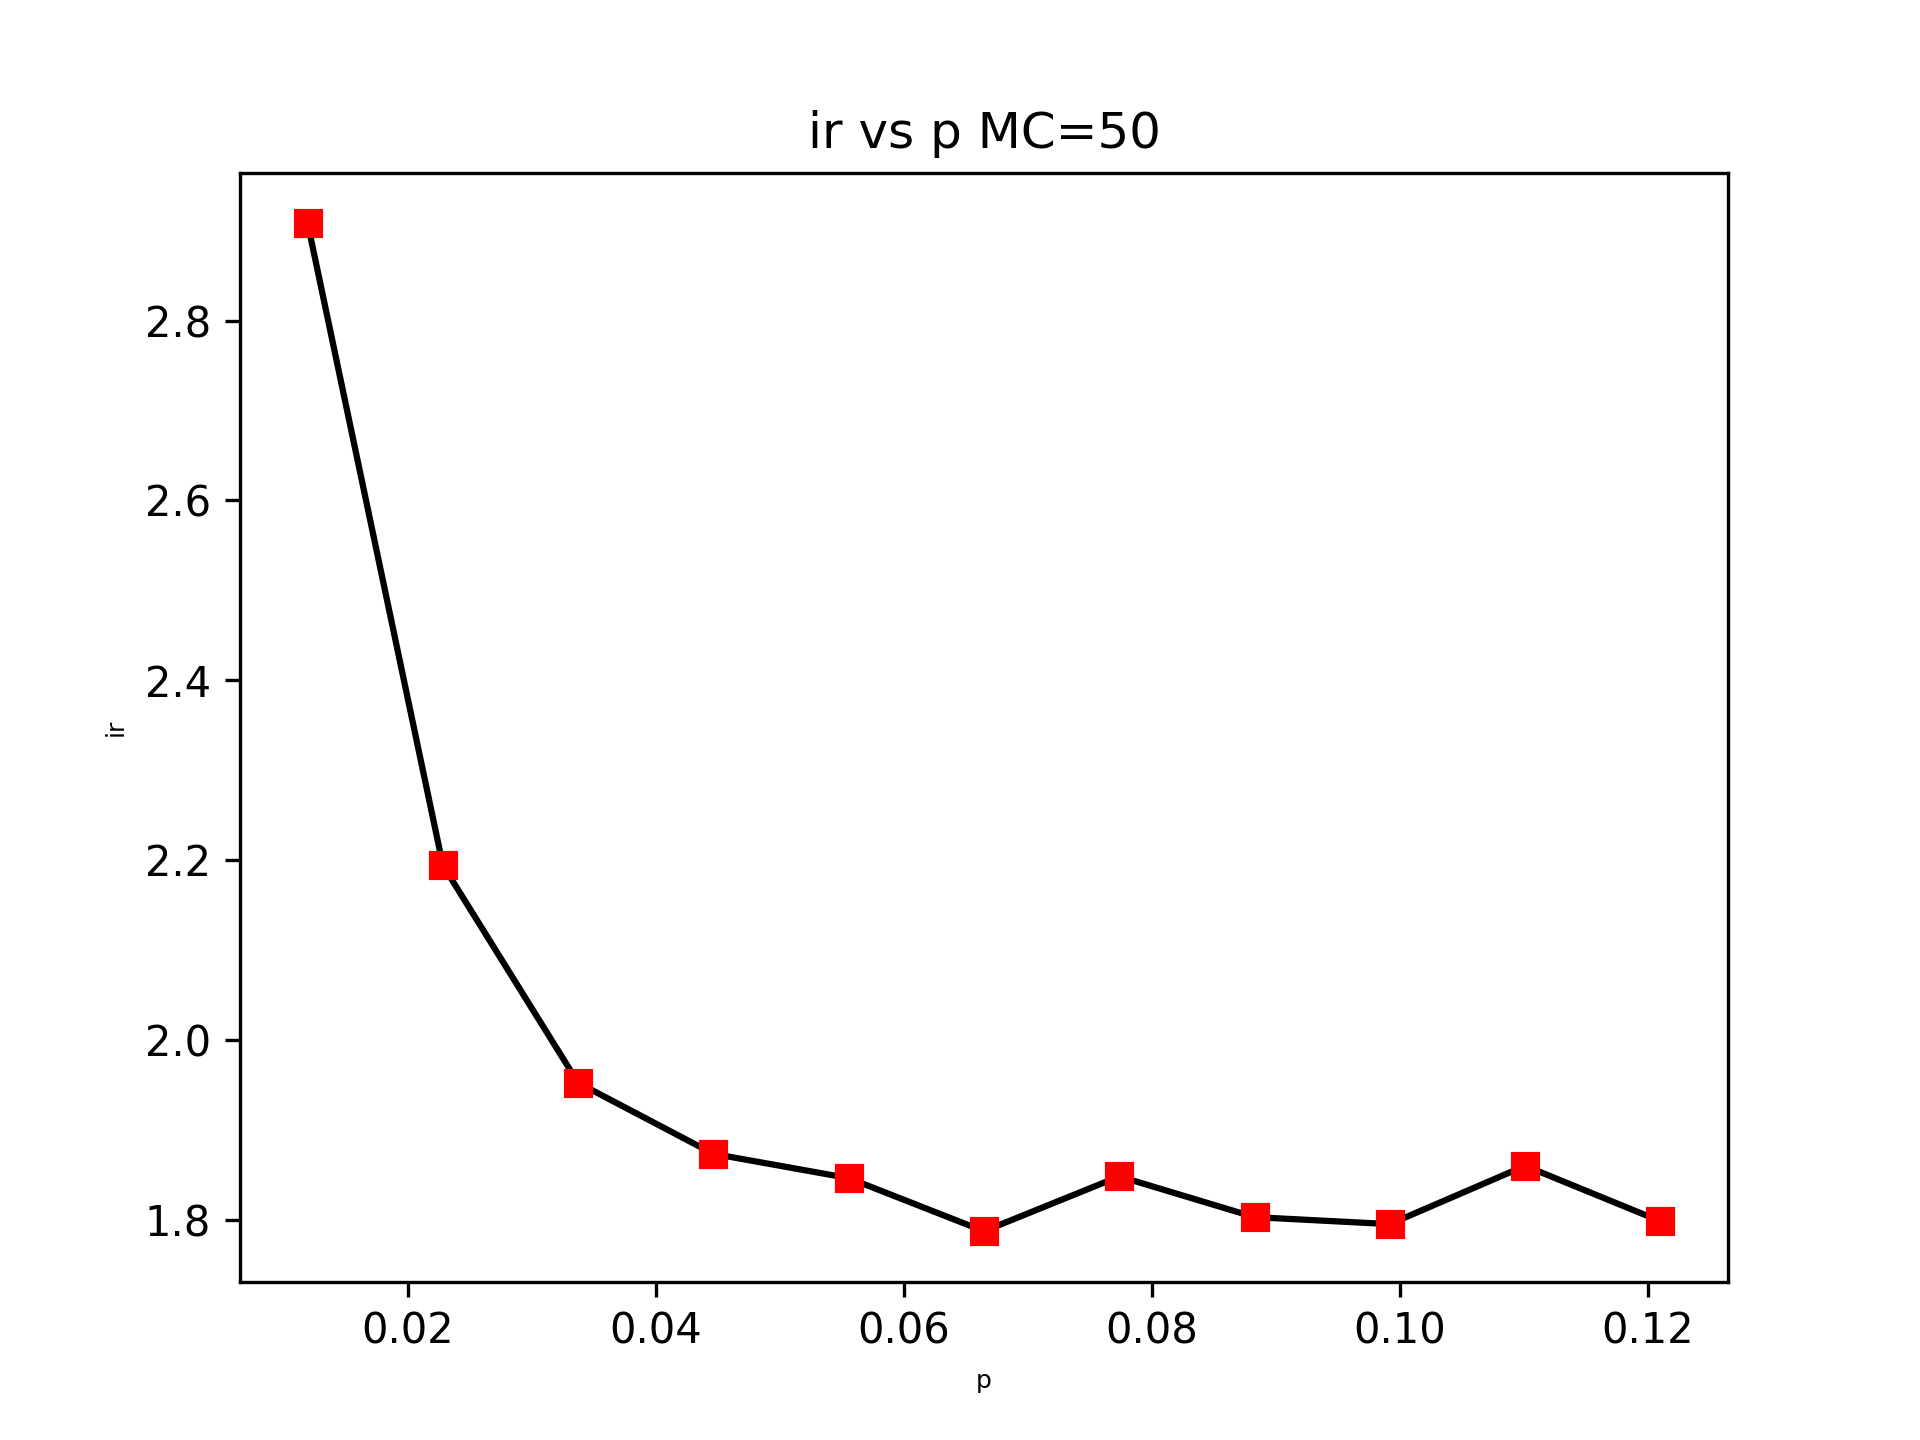
\includegraphics[width=\textwidth, trim=0 0 0 38, clip]{ir.png}
      \end{figure}
    \end{column}
    \begin{column}{0.23\textwidth}
      \centering
      \tiny\renewcommand{\arraystretch}{0.85}\setlength{\tabcolsep}{3pt}
      \begin{tabular}{lr}
        \toprule
        $p$ &  $r^i$ \\
        \midrule
        0.012 & 2.9083 \\
        0.023 & 2.1940 \\
        0.034 & 1.9521 \\
        0.045 & 1.8731 \\
        0.056 & 1.8461 \\
        0.066 & 1.7871 \\
        0.077 & 1.8480 \\
        0.088 & 1.8027 \\
        0.099 & 1.7949 \\
        0.110 & 1.8598 \\
        0.121 & 1.7982 \\
        \bottomrule
      \end{tabular}
    \end{column}
  \end{columns}
\end{frame}

\begin{frame}{Market power $\psi$}
  \tiny $\psi$ decreases as connectivity $p$ increases (more competition).  
  \begin{columns}[T]
    \begin{column}{0.75\textwidth}
            \begin{figure}
        \centering
        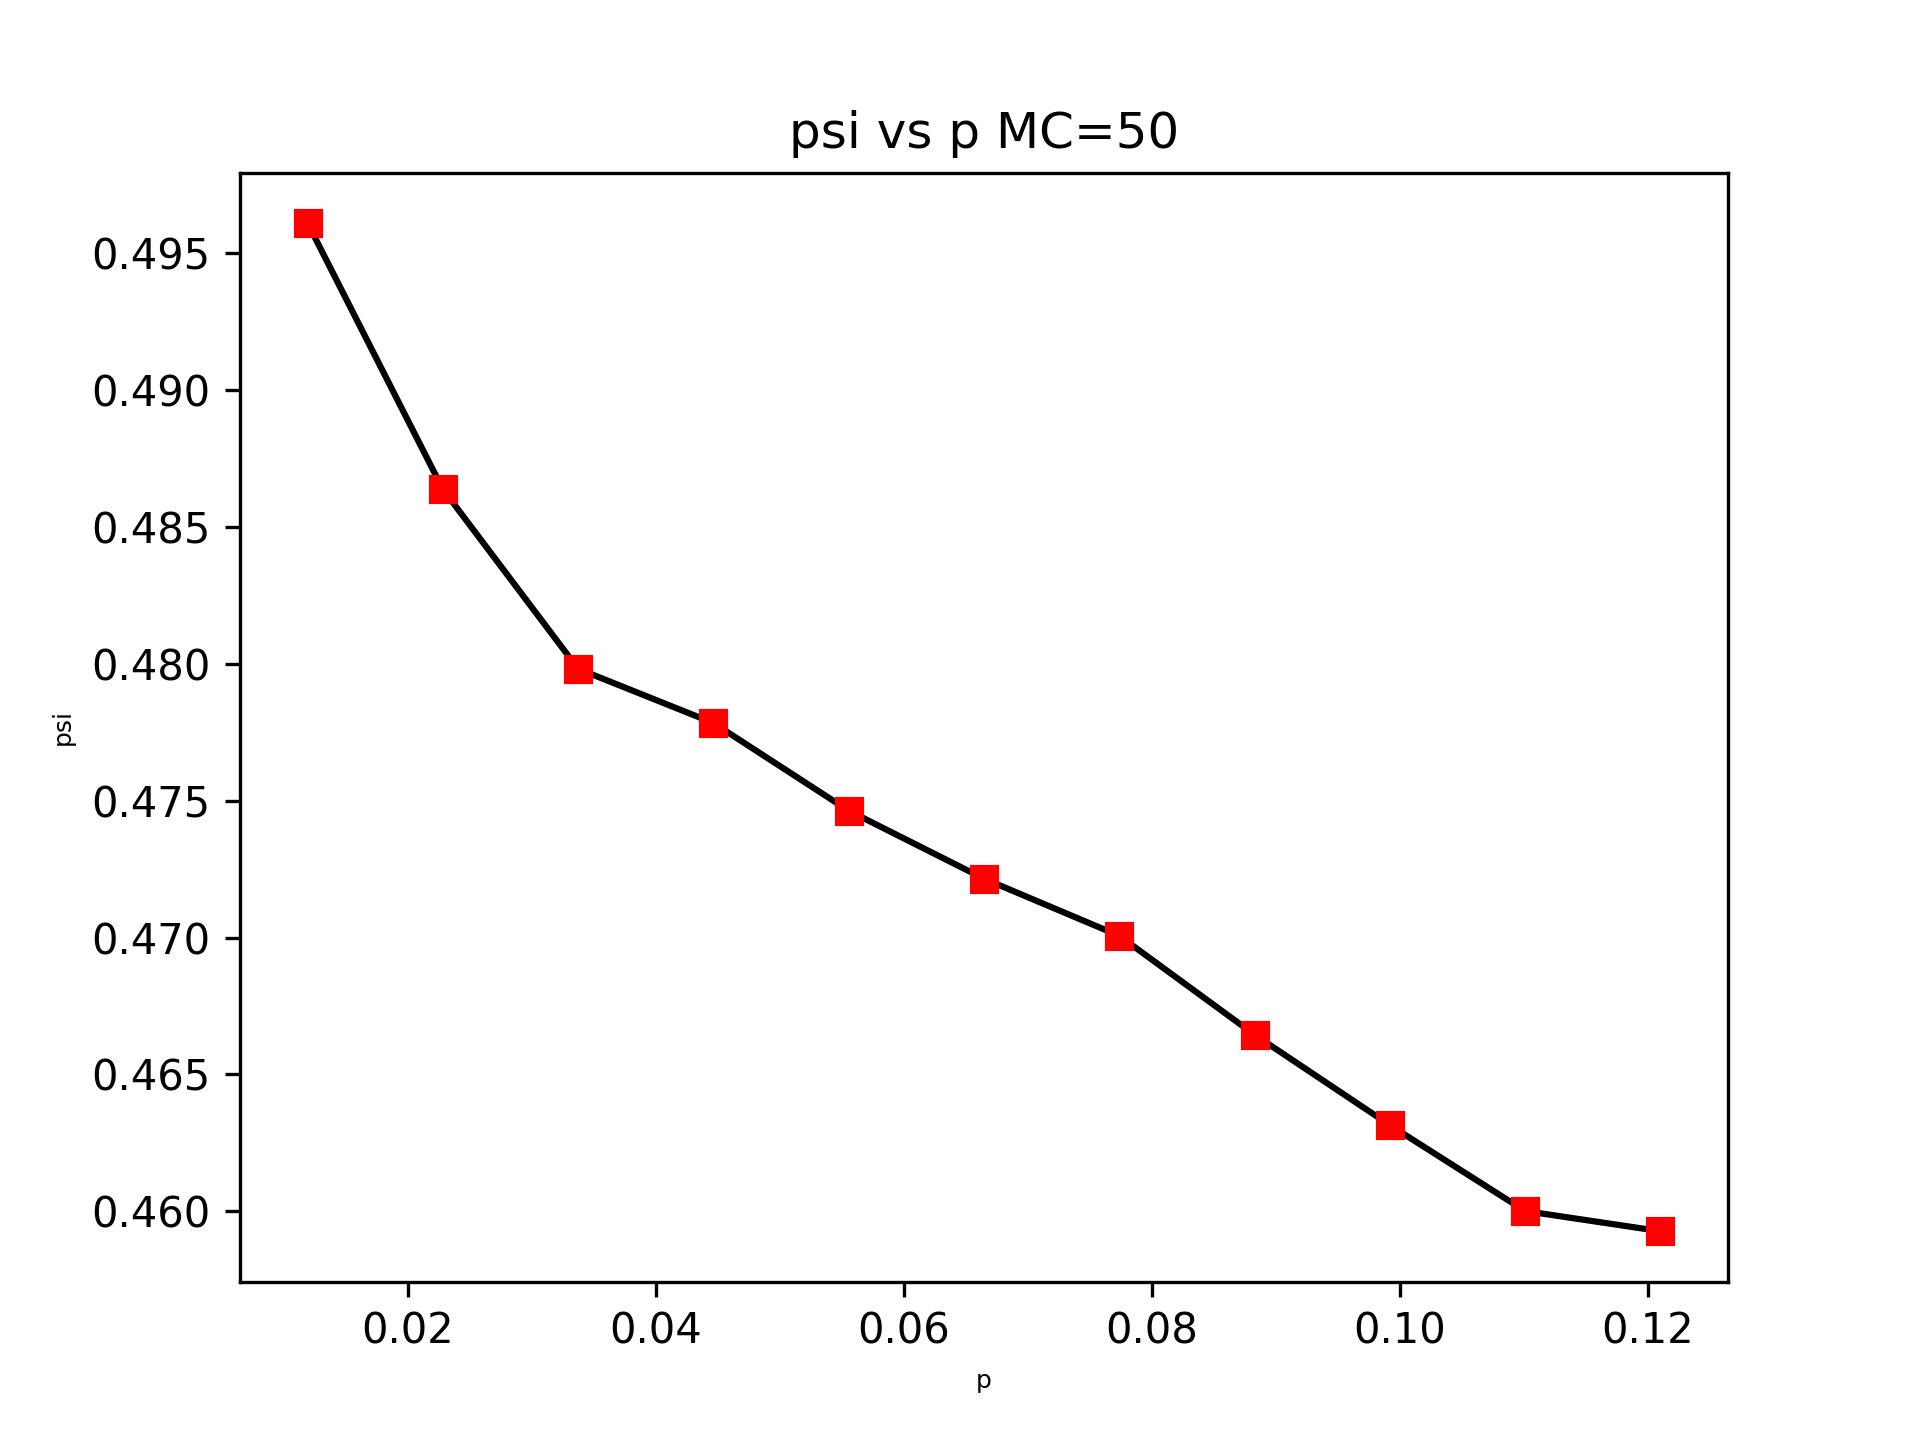
\includegraphics[width=\textwidth, trim=0 0 0 38, clip]{psi.png}
      \end{figure}
    \end{column}
    \begin{column}{0.23\textwidth}
      \centering
      \tiny\renewcommand{\arraystretch}{0.85}\setlength{\tabcolsep}{3pt}
      \begin{tabular}{lr}
        \toprule
        $p$ & $\psi$ \\
        \midrule
        0.012 & 0.4961 \\
        0.023 & 0.4864 \\
        0.034 & 0.4798 \\
        0.045 & 0.4778 \\
        0.056 & 0.4746 \\
        0.066 & 0.4721 \\
        0.077 & 0.4701 \\
        0.088 & 0.4665 \\
        0.099 & 0.4631 \\
        0.110 & 0.4600 \\
        0.121 & 0.4593 \\
        \bottomrule
      \end{tabular}
    \end{column}
  \end{columns}
\end{frame}

\begin{frame}{Probability of bankruptcy $p_b$}
  \begin{columns}[T]
    \begin{column}{0.75\textwidth}
      \begin{figure}
        \centering
        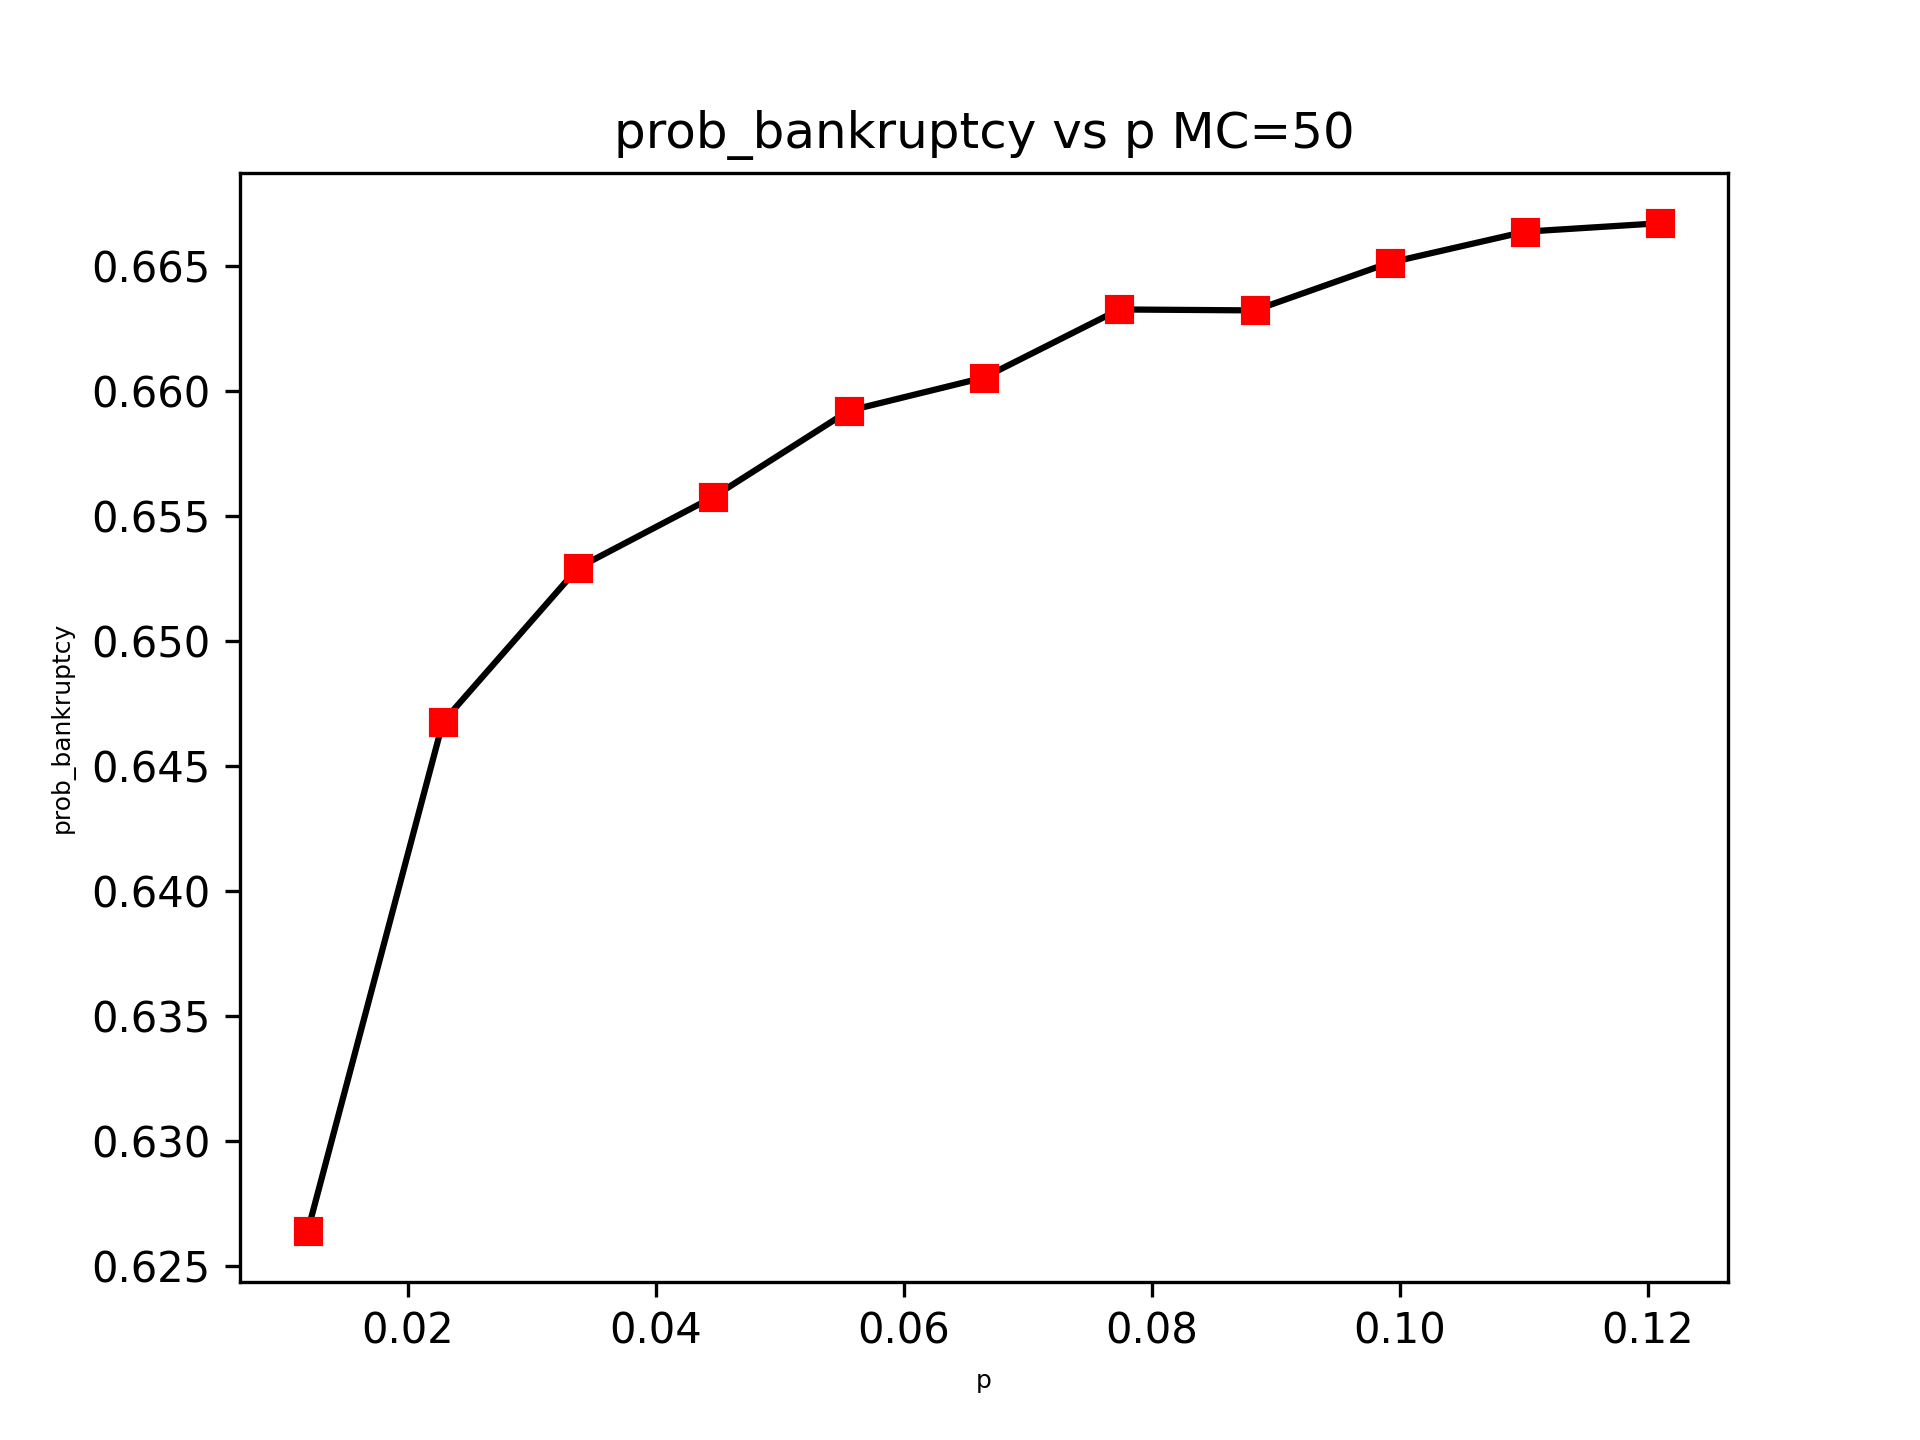
\includegraphics[width=\textwidth, trim=0 0 0 38, clip]{prob_bankruptcy.png}
      \end{figure}
    \end{column}
    \begin{column}{0.23\textwidth}
      \centering
      \tiny\renewcommand{\arraystretch}{0.85}\setlength{\tabcolsep}{3pt}
      \begin{tabular}{lr}
        \toprule
        $p$ & $p_b$\\
        \midrule
        0.012 & 0.6264 \\
        0.023 & 0.6468 \\
        0.034 & 0.6529 \\
        0.045 & 0.6558 \\
        0.056 & 0.6592 \\
        0.066 & 0.6606 \\
        0.077 & 0.6633 \\
        0.088 & 0.6632 \\
        0.099 & 0.6652 \\
        0.110 & 0.6664 \\
        0.121 & 0.6667 \\
        \bottomrule
      \end{tabular}
    \end{column}
  \end{columns}
\end{frame}

\begin{frame}{Bad debt}
  \begin{columns}[T]
    \begin{column}{0.75\textwidth}
      \begin{figure}
        \centering
        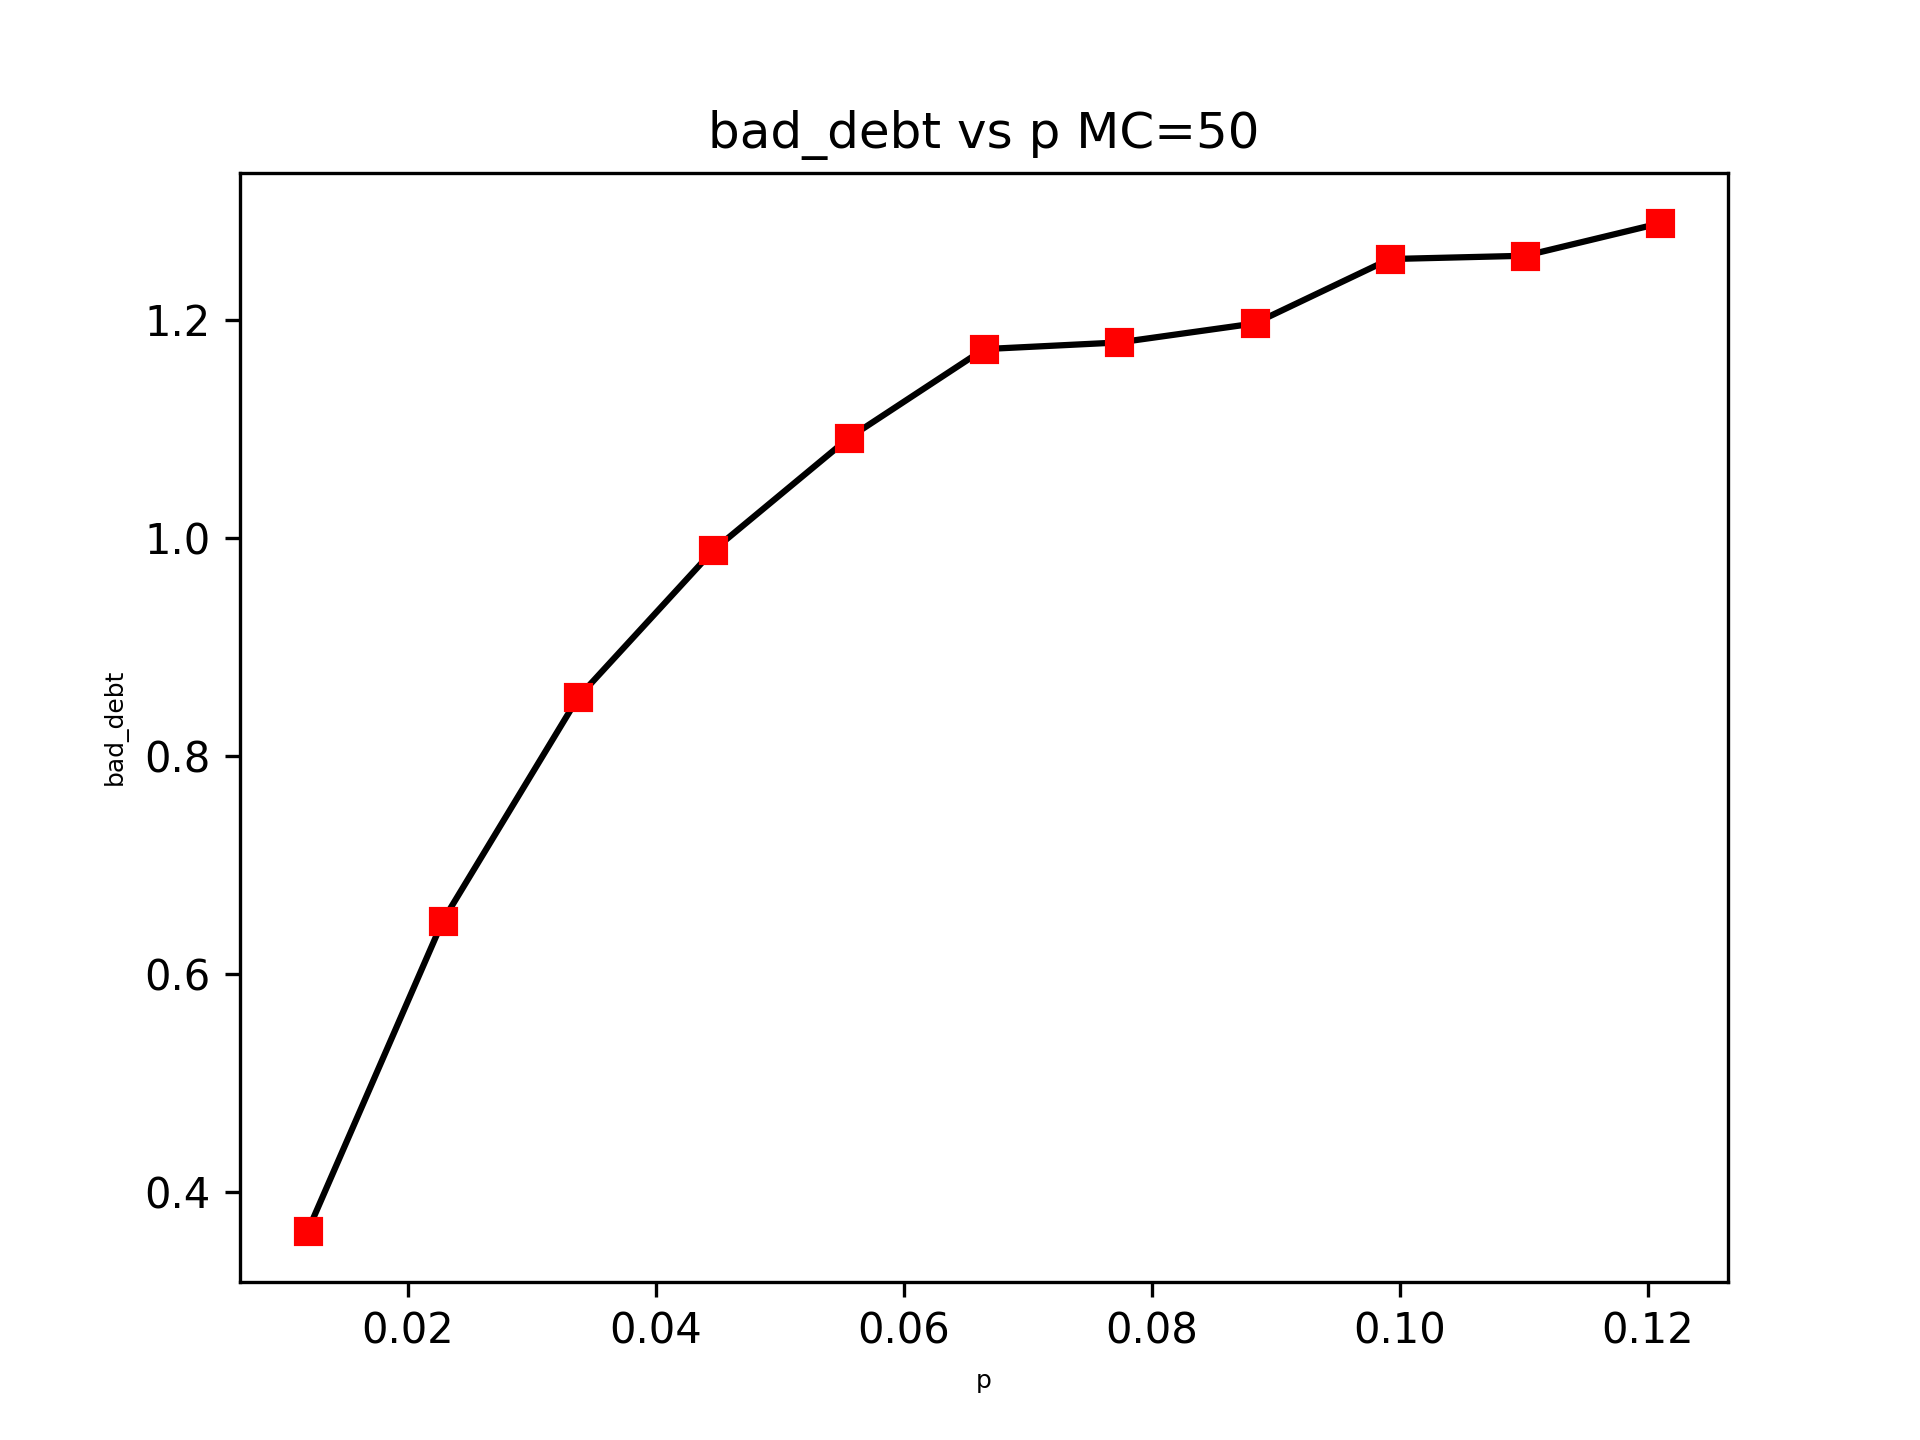
\includegraphics[width=\textwidth, trim=0 0 0 38, clip]{bad_debt.png}
      \end{figure}
    \end{column}
    \begin{column}{0.23\textwidth}
      \centering
      \tiny\renewcommand{\arraystretch}{0.85}\setlength{\tabcolsep}{3pt}
      \begin{tabular}{lr}
        \toprule
        $p$ & $B$ \\
        \midrule
        0.012 & 0.3636 \\
        0.023 & 0.6486 \\
        0.034 & 0.8536 \\
        0.045 & 0.9888 \\
        0.056 & 1.0917 \\
        0.066 & 1.1733 \\
        0.077 & 1.1794 \\
        0.088 & 1.1968 \\
        0.099 & 1.2559 \\
        0.110 & 1.2590 \\
        0.121 & 1.2888 \\
        \bottomrule
      \end{tabular}
    \end{column}
  \end{columns}
\end{frame}


%======================================================================
\section{Conclusions}\label{sec:8}
%======================================================================

\begin{frame}{Key Findings}
  As connectivity $p$ increases:
  \begin{enumerate}
    \item The Giant Component Size increases sharply above the percolation threshold.
    \item Market power decreases.
    \item The equilibrium probability of bankruptcy increases with connectivity.
    \item The equilibrium interest rate falls.
    %\item Market power has a greater effect on the interest rate than the probability of bankruptcy does.
    %\item Competition mitigates risk more effectively than isolation.
  \end{enumerate}
\end{frame}



\begin{frame}{Key Findings}
  \begin{enumerate}
    %\item \textbf{Phase transition at $p \approx 0.05$}: the network saturates and all metrics stabilize.
    \item \textbf{Failure composition shifts}: rationing dominates at low $p$; repayment failure dominates at high $p$.
    %\item \textbf{Contagion is minimal} ($<5\%$ of failures)---the dominant risk channel is business failure, not network propagation.
    %\item \textbf{Market power} ($\psi$) is positively correlated with rates and decreases as connectivity increases.
  \end{enumerate}
\end{frame}

\begin{frame}{Policy Implications}
  \begin{itemize}
    \item \textbf{Heterogeneity} is a root cause of systemic instability; the failure of large banks has disproportionate systemic effects.
    \item Interbank lending should ideally be restricted among banks with \textbf{similar liquidity characteristics}.
    \item Reserve requirements dampen cascades but \textbf{constrain growth}.
    \item Risk diversification across many agents has \textbf{ambiguous} effects on total systemic stability.
  \end{itemize}
\end{frame}

\end{document}
